\chapter{2016}
\section*{一、 选择题(本大题共 20 小题,每小题 2 分,共 40 分)}

1. 下列程序的时间复杂度为 (   )。

\begin{lstlisting}[language=C, basicstyle=\ttfamily]
i=0;s=0;n=100;
while (s<n)
{
    i++;
    s=s+i;
}
\end{lstlisting}

A) \(O\left( \sqrt{n}\right)\) B) \(O\left( \sqrt{2n}\right)\)

C) \(O\left( n\right)\) D) \(O\left( {n}^{2}\right)\)

2. 若线性表的操作主要是查找, 很少涉及到插入、删除操作时, 宜采用以下存储结构较为合适(   )。

A)双链表 B)单链表

C)顺序表 D)循环链表

3. 线性表采用链表存储时地址(   )。

A)必须是连续的 B)连续不连续都可以

C)一定是不连续的 D) 部分地址必须是连续的

4. 若允许表达式内多种括号混合嵌套, 则设计检查表达式中括号是否正确配对的算法,通常选用的辅助结构是(   )。

A) 栈 B)线性表

C) 队列 D) 二叉排序树

5. 若进栈序列为1,2,3,4,5,6,且进栈和出栈可以穿插进行,则不可能出现的出栈序列是(   )。

A)2,4,3,1,5,6 B)3,2,4,1,6,5

C)4,3,2,1,5,6 D)2,3,5,1,6,4

6. 栈和队列的共同点是(   )。

A) 都是先进先出 B) 都是先进后出

C)只允许在端点处插入和删除元素 D) 没有共同点

7. 在长度为 \(\mathrm{n}\) 的顺序表中删除第 \(\mathrm{i}\left( {1 \leq  \mathrm{i} \leq  \mathrm{n}}\right)\) 个元素时,需要移动元素的次数为 (   )。

A) n-i+1 B) i

C) i+1 D) n-i

8. 用链表作为线性表的存储结构的优点是(   )。

A) 便于随机存取 B)花费的存储空间比顺序表少

C)便于插入与删除 D)数据元素的物理顺序与逻辑顺序相同

9. 设循环队列中数组的下标范围是 0 到 n-1 ,其头指针 front 指向队首元素 rear 指向队尾元素,则队列的长度为(   )。

A) rear-front B) rear-front+1

C) (rear-front+1) \% (n-1) D) (rear-front+n+1) \%n): (   ) 0 ) (   ).

10. 二维数组 \(\mathrm{A}\left\lbrack  {12}\right\rbrack  \left\lbrack  {18}\right\rbrack\) 采用列优先的存储方法,若每个元素各占 3 个存储单元, 且 \(\mathrm{A}\left\lbrack  0\right\rbrack  \left\lbrack  0\right\rbrack\) 地址为 150 ,则元素 \(\mathrm{A}\left\lbrack  9\right\rbrack  \left\lbrack  7\right\rbrack\) 的地址为 (   )。

A) 429 B) 432

C) 435 D) 438

11. 含有 10 个结点的二叉树中, 度为 0 的结点数个数为 4 , 则度为 2 的结点个数为(   )。

A) 3 B) 4

C) 5 D) 6

12. 关于树和森林,下列说法错误的是(   )。

A)树的结点数可以为 0

B) 树的度是树内各结点的度的最大值

C) 树的子树可以有顺序, 也可以无顺序

D)二叉树不是树

13. 在一个图中,所有顶点的度数之和等于所有边数的(   )倍。

A) \(1/2\) B) 1

C) 2 D) 4

14. 如果求一个连通图中以某个顶点为根的高度最小的生成树, 应采用 (   )。

A) 深度优先搜索算法 B) 广度优先搜索算法

C)求最小生成树的普里姆算法(Prim 算法) D) 拓扑排序算法

15. 下面哪一方法可以判断出一个有向图是否有环(即回路)(   )。

A) 求节点的度 B)拓扑排序

C) 求最短路径 D) 求关键路径

16. 已知无向图的邻接表如下图所示,根据算法,则从顶点 \({\mathrm{V}}_{0}\) 出发按深度优先遍历的顶点序列是(   )。 A) \({\mathrm{V}}_{1}{\mathrm{\;V}}_{3}{\mathrm{\;V}}_{2}{\mathrm{\;V}}_{0}\) B) V0 V2 V3 V1 C) \({\mathrm{V}}_{0}{\mathrm{\;V}}_{3}{\mathrm{\;V}}_{2}{\mathrm{\;V}}_{1}\) D) \({\mathrm{V}}_{0}{\mathrm{\;V}}_{1}{\mathrm{\;V}}_{2}{\mathrm{\;V}}_{3}\) 注: 所有答案必须写在答题纸上, 试卷上作答无效 !

\begin{center}
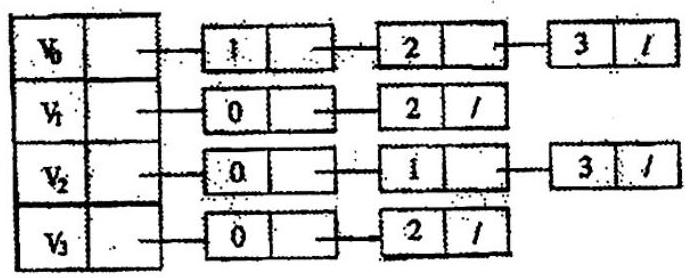
\includegraphics[width=0.5\textwidth]{images/2016/choice_16.jpg}
\end{center}
\hspace*{3em} 

17. 能进行二分查找的线性表,必须以 (   )。

A) 顺序方式存储, 且元素按关键字分块有序

B) 链式方式存储, 且元素按关键字有序

C) 顺序方式存储, 且元素按关键字有序

D) 链式方式存储, 且元素按关键字分块有序

18. 快速排序在下列哪种情况下最易发挥其长处。(   )

A) 被排序的数据中含有多个相同排序码

B) 被排序的数据已基本有序

C) 被排序的数据完全无序

D) 被排序的数据中的最大值和最小值相差悬殊

19. 非空的单循环链表的头指针为 head, 尾指针为 rear, 则下列条件成立的是 (   )。

A) rear->next->next==head B) rear->next==head

C) head->next= = rear D) head->next->next= = rear

20. 已知一个有向图如下图所示,则从顶点 \(\mathrm{a}\) 出发进行深度优先偏历,不可能得到的深度优先遍历序列为(   )。

\begin{center}
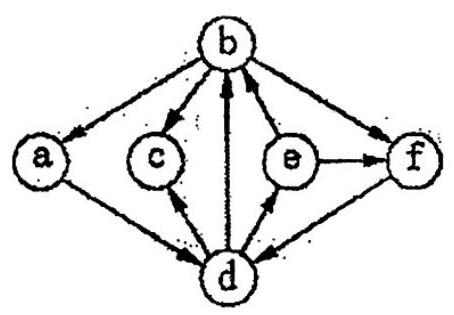
\includegraphics[width=0.3\textwidth]{images/2016/choice_20.jpg}
\end{center}
\hspace*{3em} 

A) a d b e f c

B) a d c e f b

C) a d c b f e

D) a d e f c b

\section*{二、填空题(本大题共 15 小题,每小题 2 分,共 30 分)}

1. 假设长度为 \(\mathrm{n}\) 的顺序表查找每个数据元素的概率相等,即 \({\mathrm{P}}_{\mathrm{i}} = 1/\mathrm{n}\) ,则顺序查找算法的平均查找长度为:\_\_\_\_\_\_\_\_。

2. 设指针变量 \(\mathrm{p}\) 指向单链表中结点 \(\mathrm{A}\) ,则删除结点 \(\mathrm{A}\) 的语句序列为: \(\mathrm{q} = \mathrm{p} -  > \mathrm{{next}}\) ; \(p -  >\) data \(= q -  >\) data; \(p -  >\) next \(=\) \_\_\_\_\_\_\_\_; fee(q)。

3. 设栈 \(\mathrm{S}\) 和队列 \(\mathrm{Q}\) 的初始状态为空,元素 \({\mathrm{S}}_{1},\mathrm{\;S}2,\mathrm{\;S}3,\mathrm{\;S}4,\mathrm{\;S}5,\mathrm{\;S}6\) 将依次入栈 \(\mathrm{S}\) ,一个元素出栈后即进入队列 \(\mathrm{Q}\) 。如果这 6 个元素的出队顺序为 \(\mathrm{S}2,\mathrm{S}3\) , \(\mathrm{S}4,\mathrm{S}6,\mathrm{S}5,\mathrm{S}1\) ,则栈 \(\mathrm{S}\) 的容量至少应该是\_\_\_\_\_\_\_\_,上述过程才不会错。

4. 不论是顺序存储结构的栈还是链式存储结构的栈, 其入栈和出栈操作的时间复杂度均为\_\_\_\_\_\_\_\_(要求填写大 0 表示的时间复杂度)。

5. 假定一棵树的广义表表示为 \(\mathrm{A}\left( {\mathrm{C},\mathrm{D}\left( {\mathrm{E},\mathrm{F},\mathrm{G}}\right) ,\mathrm{H}\left( {\mathrm{I},\mathrm{J}}\right) }\right)\) ,则树的深度为\_\_\_\_\_\_\_\_。

6. 设有 \(\mathrm{n}\) 个结点的完全二叉树,如果按照从自上到下、从左到右从 1 开始顺序编号,则编号为 \(\mathrm{i}\) 的节点的右孩子结点的编号为\_\_\_\_\_\_\_\_。

7. 一棵具有 257 个结点的完全二叉树,它的深度为\_\_\_\_\_\_\_\_。

8. 设某无向图中顶点数和边数分别为 \(\mathrm{n}\) 和 \(\mathrm{e}\) ,所有顶点的度数之和为 \(\mathrm{d}\) ,则 e=\_\_\_\_\_\_\_\_。

9. 具有 100 个叶子节点的哈夫曼树中,其节点总数为\_\_\_\_\_\_\_\_个。

10. 含有 12 个节点的平衡二叉树的最大深度是\_\_\_\_\_\_\_\_(设平衡二叉树的根节点的深度是 i )。

11. 设二叉树 \(\mathrm{T}\) 的前序遍历序列和中序遍历序列分别是: \(\mathrm{b},\mathrm{d},\mathrm{c},\mathrm{a},\mathrm{e},\mathrm{f}\) 和 \(\mathrm{c}\) , \(\mathrm{d},\mathrm{e},\mathrm{a},\mathrm{b},\mathrm{f}\) ; 则其后续遍历序列为\_\_\_\_\_\_\_\_。

12. 设查找表中有 100 个元素,如果用二分法查找方法查找数据元素 \(\mathrm{x}\) ,则最多需要比较\_\_\_\_\_\_\_\_ 次就可以断定数据元素 \(\mathrm{x}\) 是否在查找表中。

13. 设有一稀疏图 G,则 G 采用\_\_\_\_\_\_\_\_(若只考虑采用邻接矩阵或邻接表存储)存储较省空间。

14. 折半查找有序表(4,6,12,20,28,38,50,70,88,100),若查找表中元素20, 它将依次与表中元素\_\_\_\_\_\_\_\_ 比较大小。

15. 在插入和选择排序中,若初始数据基本正序,则选用\_\_\_\_\_\_\_\_排序。

\section*{三、问答题(本大题共 7 小题,每小题 8 分,共 56 分)}

1. 将如题图 1(a) 所示的一棵树转换为对应的二叉树, 并画出二叉树; 将图1(b) 所示的一棵二叉树转换成森林。

\begin{figure}[htbp]
    \centering
    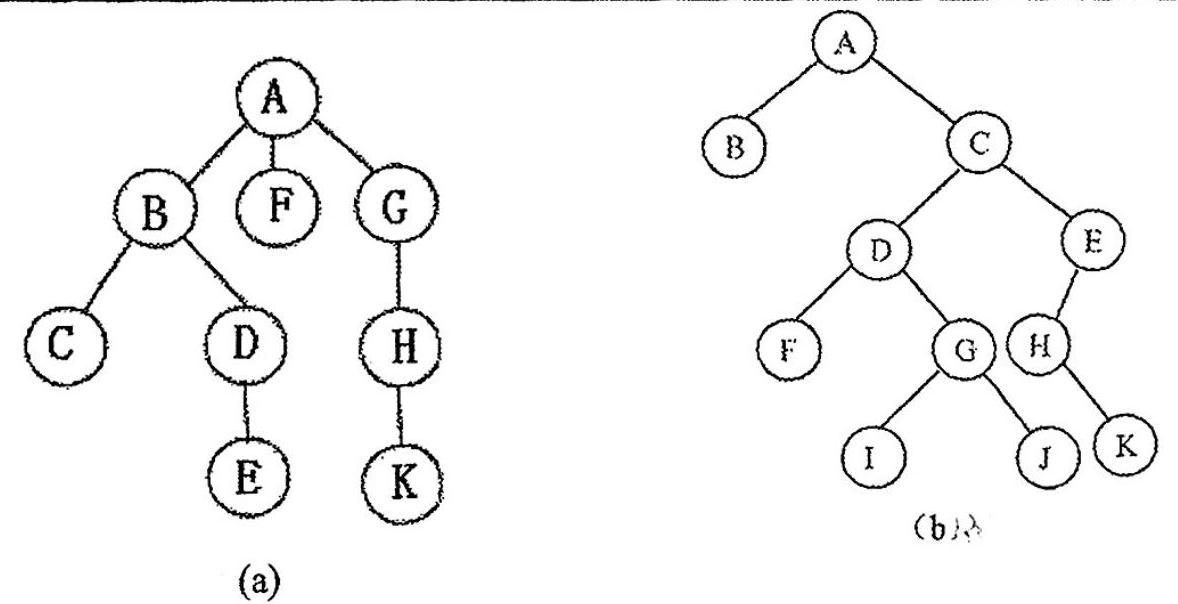
\includegraphics[width=0.3\textwidth]{images/2016/ask_1.jpg}
    \caption*{图1} % 使用带星号的 caption*
\end{figure}
\vspace{15em}

2. 如题图 2 所示有一棵二叉树, 写出该二叉树的先根遍历 (先序遍历) 序列和中根遍历 (中序遍历) 序列。

\begin{figure}[htbp]
    \centering
    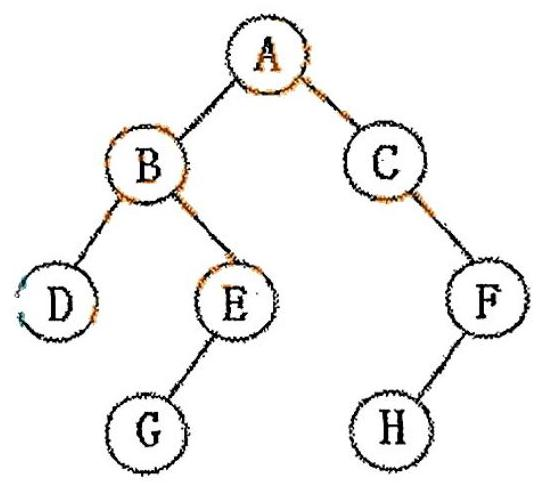
\includegraphics[width=0.3\textwidth]{images/2016/ask_2.jpg}
    \caption*{图2} % 使用带星号的 caption*
\end{figure}
\vspace{15em}

\newpage
3. 如题图 3 矩阵表示一个无向连通网 (其中 \(\infty\) 表示没有边,距离为 \(\infty\) ),试画出它所表示的连通网及该连通网的最小生成树。
\vspace{15em}

4. 如题图 4 是带权的有向图 G,画出其邻接表 (要求:邻接表中) 并根据邻接表写出其深度优先遍历序列。

\begin{figure}[htbp]
    \centering
    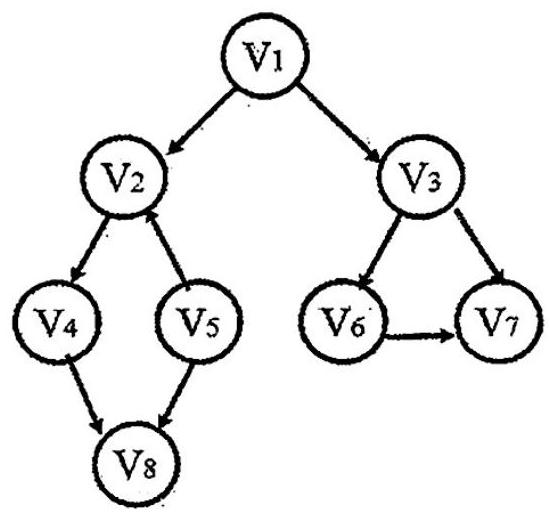
\includegraphics[width=0.3\textwidth]{images/2016/ask_4.jpg}
    \caption*{图4} % 使用带星号的 caption*
\end{figure}
\vspace{15em}

\newpage
5. 试写出一组键值(46,58,15,45,90,18,10,62)应用直接插入排序算法从小到大排序后各趟的结果。
\vspace{15em}

6. 请利用遮杰斯特拉(Dijkstra)算法求出图 5 中从顶点 \({\mathrm{V}}_{0}\) (标号为 0 的顶点) 到其他各项点间的最短路径, 请跟据表中已经完成的寻找第 1 个最短路径的点提示完成下表。

\begin{figure}[htbp]
    \centering
    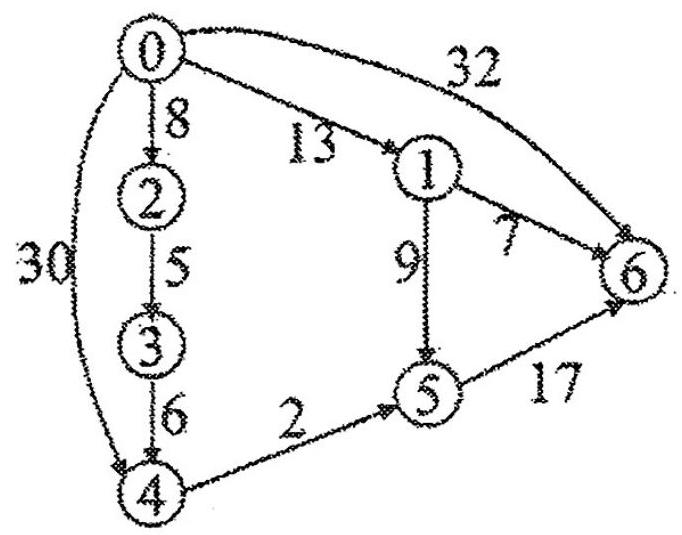
\includegraphics[width=0.3\textwidth]{images/2016/ask_6.jpg}
    \caption*{图5} % 使用带星号的 caption*
\end{figure}

\begin{center}
\begin{tabular}{|c|c|c|c|c|c|c|}
\hline
\multirow{2}{*}{终点} & \multicolumn{6}{|c|}{从 \(\mathrm{{VO}}\) 到各终点的 \(\mathrm{D}\) 值和最短路径的求解过程} \\
\cline{2-7}
 & i=1 & i=2 & i=3 & i=4 & i=5 & i=6 \\
\cline{1-7}
V1 & 13 (V0, V1) & \phantom{X} & \phantom{X} & \phantom{X} & \phantom{X} & \phantom{X} \\
\cline{1-7}
V2 & 8 (V0, V2) & \phantom{X} & \phantom{X} & \phantom{X} & \phantom{X} & \phantom{X} \\
\cline{1-7}
V3 & \(\infty\) & \phantom{X} & \phantom{X} & \phantom{X} & \phantom{X} & \phantom{X} \\
\cline{1-7}
V4 & 30 (V0, V4) & \phantom{X} & \phantom{X} & \phantom{X} & \phantom{X} & \phantom{X} \\
\cline{1-7}
V5 & \(\infty\) & \phantom{X} & \phantom{X} & \phantom{X} & \phantom{X} & \phantom{X} \\
\cline{1-7}
V6 & 32 (V0, V6) & \phantom{X} & \phantom{X} & \phantom{X} & \phantom{X} & \phantom{X} \\
\cline{1-7}
Vj & V2 . & \phantom{X} & \phantom{X} & \phantom{X} & \phantom{X} & \phantom{X} \\
\cline{1-7}
S & \(\{ {V0},{V2}\}\) & \phantom{X} & \phantom{X} & \phantom{X} & \phantom{X} & \phantom{X} \\
\cline{1-7}
\hline
\end{tabular}
\end{center}
\vspace{3em}

\newpage
7. 已知哈希函数为 \(H\left( K\right)  = \left( {3 * K}\right) {\;\operatorname{mod}\;{11}}\) ,采用线性探测再散列解决冲突 \({\mathrm{H}}_{\mathrm{i}} = \left( {\mathrm{H}\left( \mathrm{K}\right)  + \mathrm{{di}}}\right) {\;\operatorname{mod}\;\mathrm{{ll}}}\) ,对下列线性表(6,8,10,17,20,23,53,41,54,57) 求其哈希表。要求将关键字23,53,41,54和 57 依次存入到下面的哈希表中, 并填写相应的探测次数。

答: 哈希表如下:

\begin{center}
\begin{tabular}{|c|c|c|c|c|c|c|c|c|c|c|c|}
\hline
\phantom{X} & 0 & 1 & 2 & 3 & 4 & 5 & 6 & 7 & 8 & 9 & 10 \\
\cline{1-12}
哈希表 & \phantom{X} & \phantom{X} & 8 & \phantom{X} & \phantom{X} & 20 & \phantom{X} & 6 & 10 & 17 & \phantom{X} \\
\cline{1-12}
探测次数 & \phantom{X} & \phantom{X} & 1 & \phantom{X} & \phantom{X} & 1 & \phantom{X} & 1 & 1 & 3 & \phantom{X} \\
\cline{1-12}
\hline
\end{tabular}
\end{center}

\section*{四、算法设计、分析题(本大题共 2 小题,每小题 12 分,共 24 分)}

1. 请设计一个算法,将有 \(n\) 个元素的数组 \(A\) 中的元素 \(A\left\lbrack  0\right\rbrack\) 至 \(A\left\lbrack  {n - 1}\right\rbrack\) 循环右移 \(k\) 位,并要求只用一个元素大小的附加存储,元素移动或交换次数为 \(\mathrm{O}\left( \mathrm{n}\right)\) 。要求先给出算法思想, 再描述算法, 必要时请给予注释和说明。
\vspace{15em}

2. 设计在二叉排序树上查找节点的值等于 key (int 类型) 的节点算法。其中二叉树用二叉链表的形式表示, 定义如下:
\begin{lstlisting}[language=C, basicstyle=\ttfamily]
typedef struct node{
    int key;
    struct node *lchild,*rchild;
}BinNode,*bitree;
\end{lstlisting}


要求先给出算法思想,再描述算法,必要时请给予注释和说明。